\chapter{Implementation}
\label{cha:implementation}

The final implementation of our system is as follows [\ref{fig:architecture2}]:
\begin{figure}[h!]
\centering
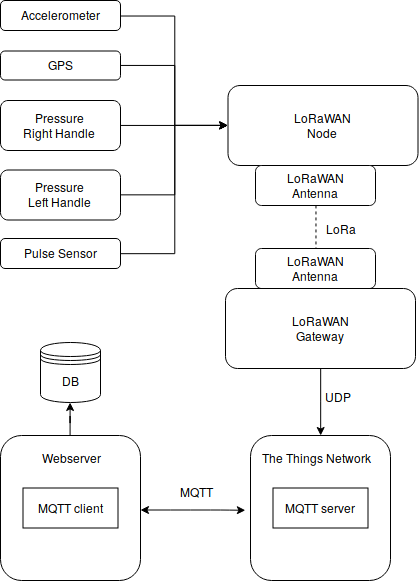
\includegraphics[width=1\linewidth]{gfx/architecture_implementation_h}
\caption{Implemented Architecture}
\label{fig:architecture2}
\end{figure}

It differed from the proposed design in the following ways:

We decided to use a webserver with an mqtt client and a database instead of a central server with API. We also decided to not implement the analytics server as part of the current project. We made these decisions prioritising the components that we needed to test our hypothesis. Since the presence or absence of a central server or analytics platform don't affect the parameters we need to test our hypothesis we decided to ignore them in the implementation part.


\section{Node and Gateway hardware}
	The presented architecture can be realized in a number of ways, meaning we had to make the following choices before going into details:

	\begin{itemize}
		\item Use sensors with inbuilt LoRa functionality or use a single-board computer connected to sensors and LoRa transmitter?
		\item What hardware to use to interface with the sensors and act as the node?
		\item What hardware to use as LoRaWAN gateway?
	\end{itemize}


	\subsection{Single-board Computer vs Inbuilt LoRa Sensors}

		We had the option of using a single-board computer (SBC) to interface with all of the sensors (Arduino or Rpi) or using sensors with inbuilt LoRaWAN capabilities.

		We summarized the characteristics of sensors with inbuilt LoRaWAN as follows:
		\begin{itemize}
			\item They require little to no configuration and work out of the box. This means using them would grant us more time to we can focus on other parts of the project.
			\item Data can be sent at different rates for each sensor.
			\item They are much more expensive than standard sensors.
			\item They are bulkier than standard sensors, making them harder to fit into the walker.
			\item Their is low variety when it comes to such sensors in the market, limiting choice of vendor and sensors.
			\item Having several LoRaWAN transmitters instead of one would make the power consumption higher.
			\item Each sensor usually has its own battery or charging method, which makes recharging more complex
		\end{itemize}


		We summarized the following characteristics of SBCs:
		\begin{itemize}
			\item Fine grained control of the sensors
			\item We might want to do some preprocessing of the sensor data before sending it, which is possible with SBCs.
			\item Good amount of variety in the market allowing us a lot of choice.
		\end{itemize}

		We decided to go with an SBC because we value the flexibility provided by the vast array of sensors to choose from and the possibility to manually program them.



	\subsection{Comparing Raspberry Pi and Arduino}

		We then had the option of either using a Raspberry Pi or an Arduino. We summarized their characteristics as follows:

		Pi:
		\begin{itemize}
			\item Faster and more powerful processor
			\item Overhead of operating system, hdmi output, wifi/ethernet port, audio output, all of which take physical or disk space.
			\item More power consumption
		\end{itemize}

		Arduino:
		\begin{itemize}
			\item Easy to get up and running
			\item Easier to connect with analog sensors
			\item Lots of different models to choose from, meaning we can choose the one that best fits our goals
			\item Cheaper than the Raspberry Pi
			\item Smaller 
			\item No operating system, meaning we are closer to the hardware and have more control over the sensors
		\end{itemize}

		Due to the points mentioned above, especially due to its flexibility, and low power consumption, we decided to go with the Arduino as the node.

		Due to its superior computational power, inbuilt networking capabilities, we decided to go with the Raspberry Pi as the gateway.

		Our reasoning is supported by the arguments put forward in \cite{postolache2011smart}.





The specifics of the implementation of each component of our system is described in detail in the following sections.


\section{Node} 
	\subsection{Hardware}
		As mentioned, the node consists of an Arduino Mega (R3 ATmega2560) with a Seeedstudio Dragino Lora Shield (868 M Frequency). It is powered by a standard 9V battery pack. The node also consists of a breadboard, which contains two Analog to Digital converter and a GPS Sensor. The entire node setup is mounted on the front face of the lower left leg of the walker. The accelerometer is directly connected to the Arduino and is mounted on the back face of the left leg of walker. Two pressure sensors are mounted on the handles of the walker and are connected to the A/D converters in the breadboard, which in turn are connected to the Arduino. The pulse sensor is mounted on the left handle and is directly connected to the Arduino.

		The circuit diagram of the node is as follows [\ref{fig:architecture_node}]:

		\begin{figure}[h!]
			\centering
			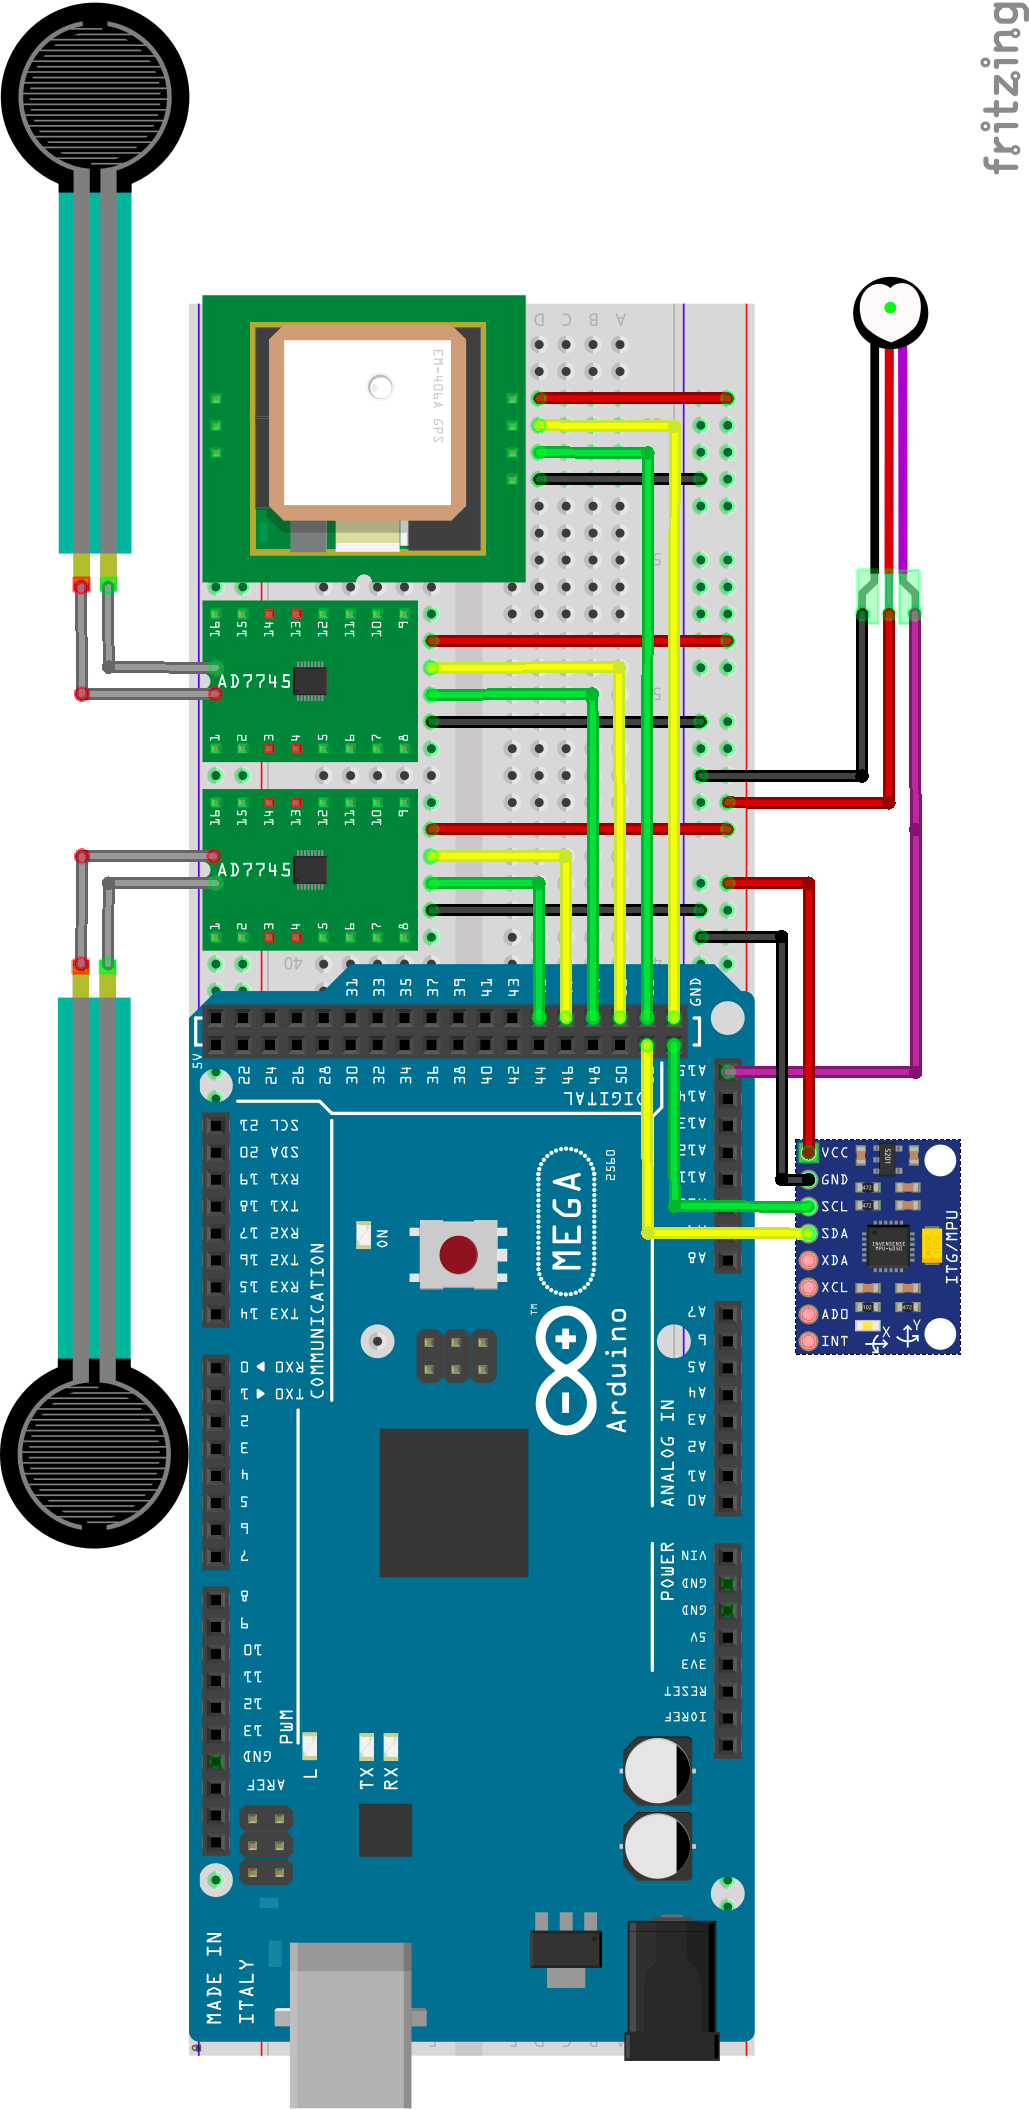
\includegraphics[width=0.7\linewidth]{gfx/node_diagram}
			\caption{Implemented Architecture ot the Node}
			\label{fig:architecture_node}
		\end{figure}
		
		The Blueprint table shows how we connected the sensors to the pins of our Arduino board [\ref{tab:blueprintArduino}]:
		\begin{table}[h!]
			\centering
			\begin{tabular}{l|ll}
				\textbf{Sensor} & \textbf{Out\_Sensor} & \textbf{In\_Arduino} \\\hline
				\textit{GPS} & VCC & 5V \\
				& RX & D12 \\
				& TX & D13 \\
				& GND & GND \\\hline
				\textit{Pressure Right} & VCC & 5V \\
				& SCK & D37 \\
				& DT & D36 \\
				& GND & GND \\\hline
				\textit{Pressure Left} & VCC & 5V \\
				& SCK & D35 \\
				& DT & D34 \\
				& GND & GND \\\hline
				\textit{Movement} & VCC & 5V \\
				& GND & GND \\
				& SCL & SCL \\
				& SDA & SDA \\\hline
				\textit{Pulse} & VCC & 5V \\
				& GND & GND \\
				& S & A15 
			\end{tabular}
			\caption[Blueprint connections node]{A: Analog, D: Digital}
			\label{tab:blueprintArduino}
		\end{table}

	\subsection{Software}
		The IDE used for writing and uploading the code was Visual Studio with Platform I/O extension. The Platform I/O simplified the process of uploading the code and monitoring the output of the Arduino mega.

		The libraries used were lmic, hal, SPI, SoftwareSerial, MPU9250 and HX711 along with the standard Arduino,stdlib and string library.

		The folder structure of the Arduino is defined in the appendix [\ref{lst:codehierarchy}]. 

		Every 15 seconds, the Arduino checks if the walker is moving through the accelerometer, and if so, polls all the other sensors by using their respective libraries, packages them into a buffer, and tries to send them over LoRaWAN.

		Each LoRaWAN packet contains its application and network keys and the device's address, which are required by The Things Network.

\section{Pressure}
	\subsection{Hardware}
	For measuring pressure we used two Aluminum Alloy pressure sensors, which have a measurement range of -10 to 10 kg, connected to the Arduino via an HX711 AD converter module. 

	\subsection{Software}
	The sensor data was collected using the HX711 library to transform the analog signal along with the standard Arduino library. 

\section{Pulse}

	\subsection{Hardware}
	For pulse, we used the pulse sensor from pulsesensor.com. It contains an LED that shines light into the capillary tissue, and the sensor reads the light that bounces back.

	\subsection{Software}
	For reading the data from the sensor, we simply read the analog input. This data is then processed to get the average heart rate of the patient by finding its pattern in the raw data.

\section{Accelerometer}

	\subsection{Hardware}
	We used an MPU9250 accelerometer to measure whether the walker is moving or not.

	\subsection{Software}
	The library used to read the accelerometer's output was the sensor specific MPU9250 library. If the gyroscope reading from the accelerometer increased beyond a certain threshold, the walker was considered to be moving.

\section{GPS}

	\subsection{Hardware}
	For measuring GPS we used the GY-GPS6MV2 sensor.

	\subsection{Software}
	The library used to read GPS data was SoftwareSerial and it was then parsed to get the value of latitude and longitude.

\section{Gateway}
		
	\subsection{Hardware}
	The gateway consists of a Raspberry Pi 3+ with a Dragino LoRa hat for Pi. The Pi was connected to a router which in turn was connected to the internet.


	\subsection{Software}
	The Raspberry Pi is running a single channel packet forwarder written in C++, which forwards the packets it receives from the node to The Things Network's european router. 

\section{The Things Network (TTN)}
	We describe our reasoning behind using TTN in the previous section [\ref{ttn_description}].

	The application in TTN receives packets from the gateway, decodes the byte array in the payload to strings and puts them into a JSON object, which is then published using the mqtt broker.

\section{Webserver}
	We created a webserver using the Django framework. It contains an mqtt client implemented using the paho-mqtt library which subscribes to our TTN application on startup. The client than waits for the TTN broker to send it the published information, which it then stores in an sqlite database and displays on the webpage using the django-tabular library.

	We chose to use the Django framework with sqlite as the database for our server, because they allow for quick prototyping and testing.

%%% Local Variables:
%%% mode: latex
%%% TeX-master: "../ClassicThesis"
%%% End:
